%------------------------ Packages ------------------------
\documentclass[12pt,a4paper]{article}
\usepackage[latin1]{inputenc}
\usepackage[T1]{fontenc}
\usepackage[pdftex]{graphicx}
\usepackage{float}
\usepackage{amsmath}
\usepackage{amssymb}
\usepackage[FIGTOPCAP]{subfigure}
\usepackage{color}
\usepackage[hidelinks]{hyperref}

\newcommand{\version}{\IfFileExists{../../version.txt}
{\input{../../version.txt}}
{\input{../../../version.txt}}
}

\newcommand{\command}[1]{%
\indent \fcolorbox{black}{white}{%
   \begin{minipage}{\dimexpr\textwidth-\parindent\relax}%
      #1
   \end{minipage}%
}
}

\newsavebox{\FVerbBox}
\newenvironment{sample}
{\par \vspace{0.2cm} \begin{lrbox}{\FVerbBox}
\begin{minipage}{\dimexpr\textwidth-\parindent\relax}}
{\end{minipage}
\end{lrbox}
\fcolorbox{black}{lightgray}{\usebox{\FVerbBox}}
\vspace{0.2cm}}

\newenvironment{sampletitle}
{\vspace{0.2cm} \noindent\textbf{Example} :
\begin{sample}}
{\end{sample}}

\newcommand{\samplecomment}[1]{%

\textit{#1}
}

\newcommand{\seealso}[1]{\vspace{0.2cm} \noindent\textbf{See also} :\par #1}

% tikz
\usetikzlibrary{calc}
\usetikzlibrary{arrows}
\usetikzlibrary{shadows}

\tikzset{block/.style={draw, text centered, fill=gray!10,drop shadow}}
\tikzset{connect/.style={draw, line width=1 pt}}

\begin{document}

\begin{center}
\textbf{\huge  \underline{Detectroi operator}}
\end{center}
\vspace{0.5cm}

The detectroi operator is a segmentation operator used to identify the knowledge rich part of an incoming binary image. With the assumption that the binary image has been stripped of all noises, the region of interest returned by this operator is defined as the smallest rectangle containing all the image white pixels.\\

The rectangle coordinates are sent on a serial format via a 64 bits frame, with the following disposition: \\
\begin{center}
$<x,y,w,h>$\\
\end{center}
Each component is 16 bits wide and the sending order is left to right, Less Significant Byte first.

\begin{figure}[h!]
\centering
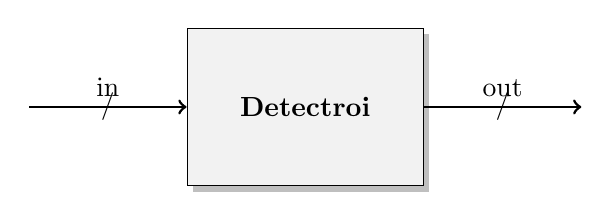
\begin{tikzpicture}
\node[block,rectangle,minimum height=2cm,minimum width=3cm] (bloc) {\textbf{Detectroi}};

\path[connect,<-] ([yshift=0.0cm]bloc.west) -- node{/} node[above]{in} ++(-2cm,0);

\path[connect,->] ([yshift=0.0cm]bloc.east) -- node{/} node[above]{out} ++(2cm,0);
 ([xshift=0.5cm,yshift=-0.6cm]bloc.north);

\end{tikzpicture}
\end{figure}


\section*{Properties}
\properties{
enable           & bool & Enable the processing \\ 
}

\vspace{0.5cm}

\section*{Constants}

\constants{
IN\_SIZE & Size of the input flow : 1 byte (greyscale image) or 1 bit (binary image)\\
OUT\_SIZE & Size of the output flow : 1 byte (greyscale image) or 1 bit (binary image)\\
}

\newpage
\section*{Mathematical formalism}

The operator initializes 4 variables $x_{min}$, $y_{min}$, $x_{max}$ and $y_{max}$ containing measured extrema for $x$ and $y$ coordinates, and update these variables for each non black pixel of the incoming binary image. The coordinates are then processed with the following rules:

\centering
$x = x_{min}$ \hspace*{2cm} $y = y_{min}$\\
$w = x_{max} - x_{min}$ \hspace*{2cm} $h = y_{max} - y_{min}$\\

\section*{Usage}
The following gpnode project uses detectroi output to display a rectangle on the original image:
\begin{figure}[h!]
\centering
\label{detectROIusage}
\caption{Model project using detectroi bloc}
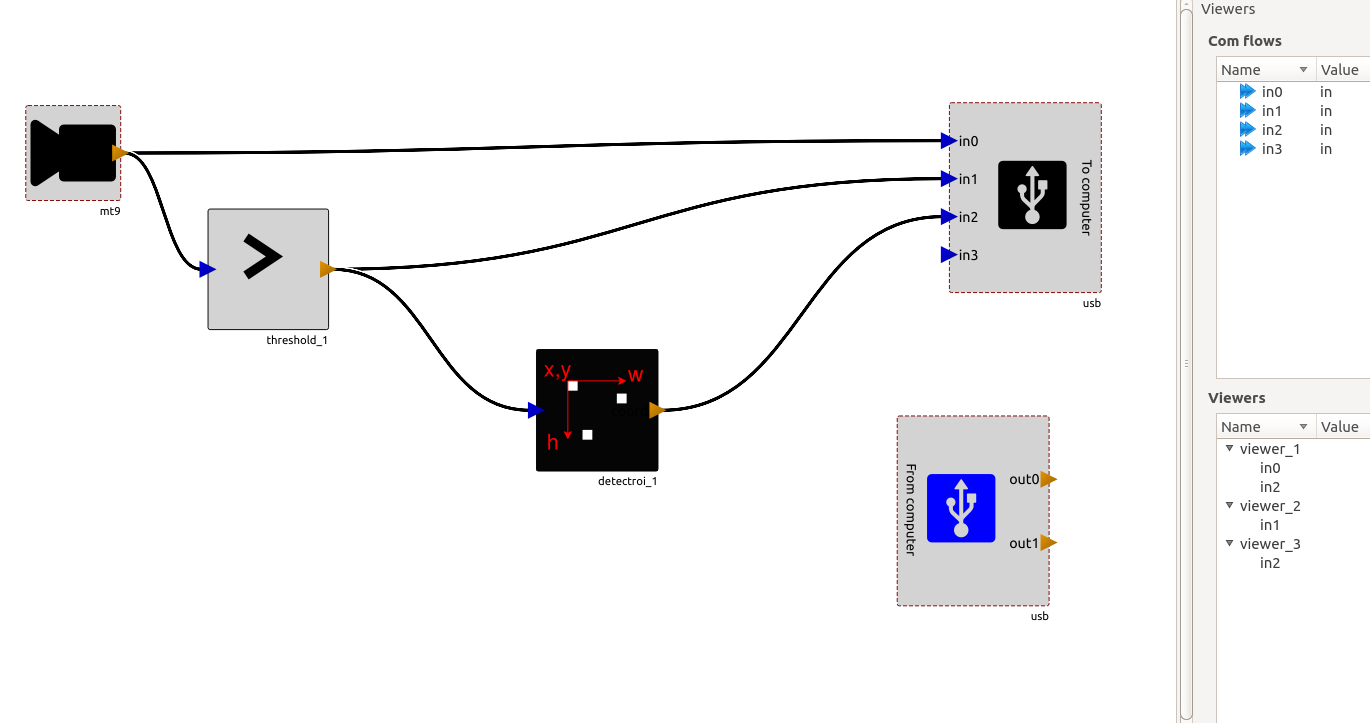
\includegraphics[width=14cm]{detectroiUsage.png}
\end{figure}

In the viewer tab, the rectangle overlay can be set with the creation of a viewer containing both image flow and rectangle flow. On the Figure \ref{detectROIusage}, $in0$ and $in2$. The observed output on gpviewer can be seen below: \\
\newpage
\begin{figure}[!h]
\centering
\subfigure[Binary image used by detectroi]{

\includegraphics[width=14cm]{binary.png}}
\subfigure[Original image with received rectangle from detectROI]{
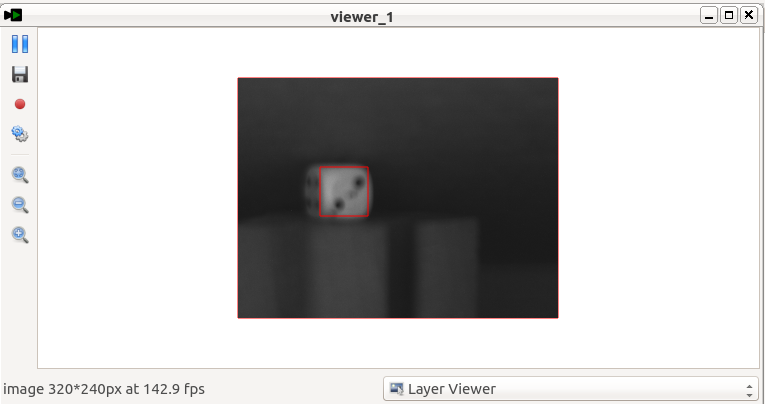
\includegraphics[width=14cm]{detected.png}}
\end{figure}


\end{document}